\section{Handling $\mu$ dependency} 

\paragraph{Metabolic constraint ($C_1$)} Let us start from the condensed form of RBA described above.

\[
[S, -\mu C_E, -\mu C_R, -\mu C_C][\nu;E;R;C] = \mu [C_G,C_{X_c}][P_G;X_c]
\]

We would like to rewrite this in the form $(A_{eq} + \mu B_{eq})[\nu;E;R;C] = c_{eq} + \mu d_{eq}$. Naively, the equation becomes

\[
([S, 0,0,0] + \mu [0, -C_E,-C_R,-C_C])[\nu;E;R;C] = \mu [C_G,C_{X_c}] [P_G;X_c]
\]

However, it is noteworthy that some terms within these matrices depend on $\mu$. \textit{A priori}, only $P_G$ is modified. In the current version, $P_G$ has 3 components: cytosolic proteins, membrane proteins, external proteins. The total number of proteins has the form $a_{tot}+b_{tot}\mu$. Then, the fraction of proteins alotted to $P_G$ is also an affine function of $\mu$. For example, the first component of $P_G$ reprensenting proteins in the cytosol is
\[
f_{cyt} (a_{tot} + b_{tot} \mu)(a_{cyt} + b_{cyt}\mu) 
= f_{cyt} (a_{tot} a_{cyt} + \mu (a_{cyt}b_{tot}+a_{tot}b_{cyt})+ \mu^2 b_{tot} b_{cyt})
\]
where $f_{cyt}$ is the fraction of proteins in the cytosol. Because this expression has only be applied to 3 terms, there is no need to use it in the general expression above. It would lead to a complex equation with dependencys up to $\mu^3$, which would be a waste of time for only 3 terms.

The other metabolic constraint writes
\[
  [I,-\diag{k_E};-I,-\diag{k_E}][\nu;E] \leq 0
\]
Here the $k_E$ are actually $\mu$-dependent. $(k_E)_i$ can be rewritten $a_i+b_i\mu$. More generally
\[
\diag{k_E} =\diag{a_{k_E}} + \mu\diag{b_{k_E}}
\]
In the end, the constraint becomes
\[
([I,-\diag{a_{k_E}};-I,-\diag{a_{k_E}}]
+ \mu [0,-\diag{b_{k_E}};0,-\diag{b_{k_E}}])
[\nu; E] \leq 0
\]

\paragraph{Other processes} 
In order to assess the $\mu$-dependency of other constraints, we need to provide a general framework for other constraints. What are the variables? The targets? Generally speaking, it feels like the variables can be any of the variables in the $[\nu; E; R; C]$ vector. Existing constraints display different behaviors. ATP maintenance is of the form
\[
A [\nu; E; R; C] \leq b + \mu c
\]
Translation is of the form
\[
(A+\mu B) [\nu;E;R;C] \leq \mu c
\]
Tthe general form is similar to the metabolic constraint
\[
(A+\mu B) [\nu;E;R;C] \leq c + \mu d
\]
In existing processes, the $\mu$-dependency comes from dilution compensation ($\mu B$ part) and parameter scaling ($\mu d$ part in the flagella and ATP maintenance processes). At the time being, I feel like it is necessary to account explicitely for dilution in the algorithm. However, $\mu$ dependency in the constant part is maybe not necessary.

\begin{figure}[ht]
  \centering
  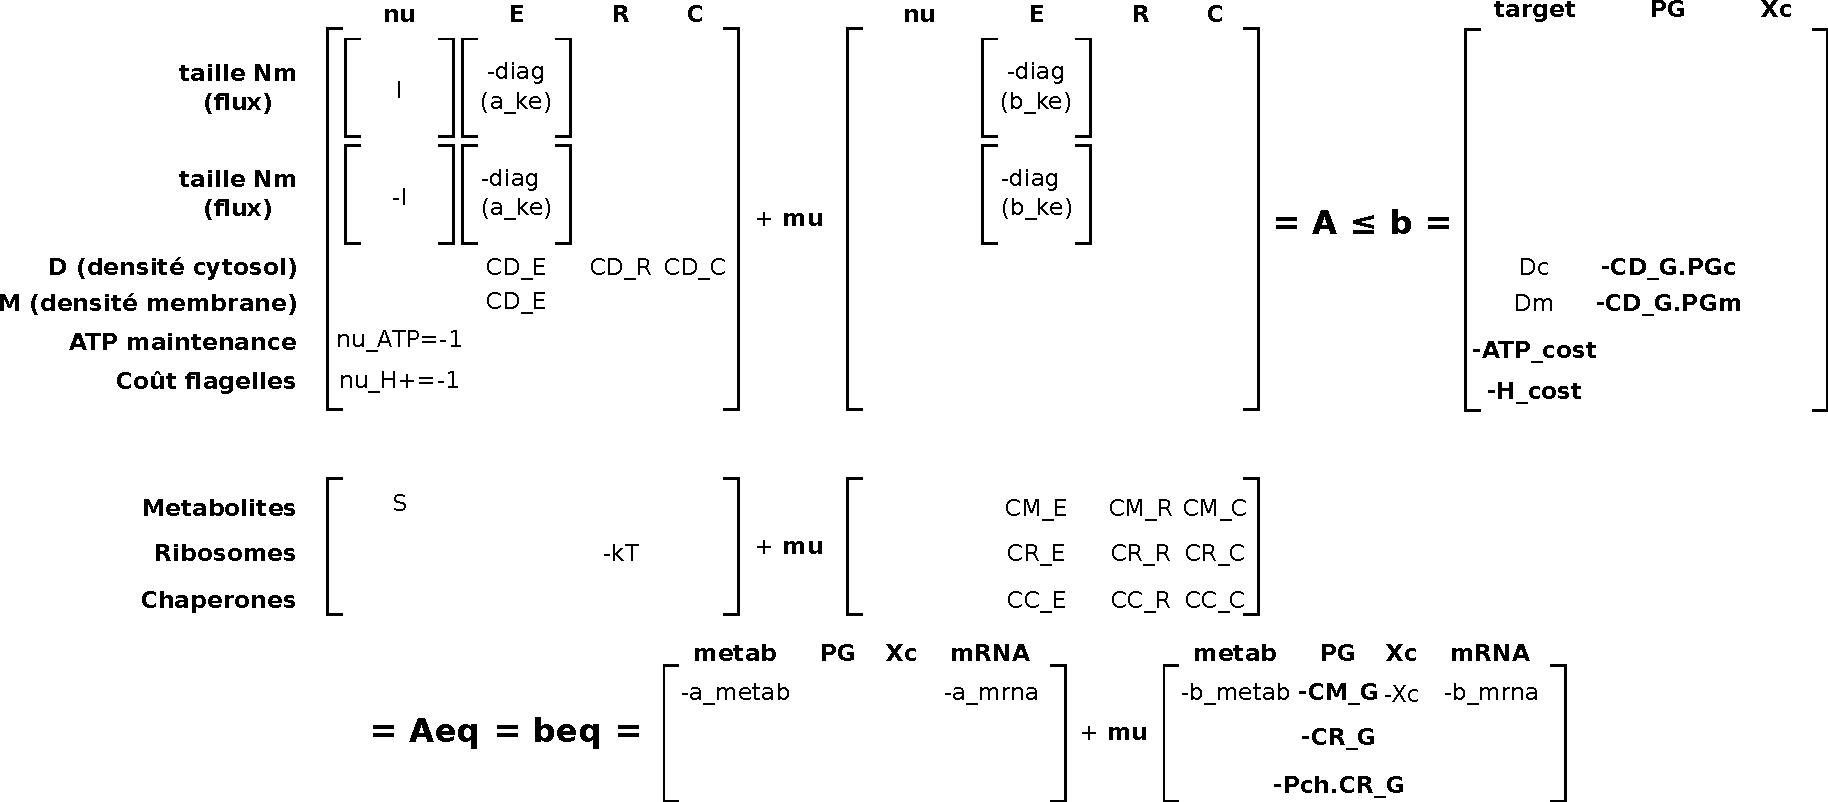
\includegraphics[width=\linewidth]{new_matrices_RBA_mu}
  \caption{Structure of matrices displaying $\mu$-dependency. All terms shown in bold depend on $\mu$.}
  \label{fig:new_matrices_rba_mu}
\end{figure}

\paragraph{Summary} 
Metabolic constraint:
\[
([S, 0,0,0] + \mu [0, -C_E,-C_R,-C_C])[\nu;E;R;C] = \mu [C_G,C_{X_c}] [P_G;X_c]
\]
Flux constraint:
\[
([I,-\diag{a_{k_E}};-I,-\diag{a_{k_E}}]
+ \mu [0,-\diag{b_{k_E}};0,-\diag{b_{k_E}}])
[\nu; E] \leq 0
\]
Other processes:
\[
(A+\mu B) [\nu;E;R;C] \leq c + \mu d
\]
\reffigt{fig:new_matrices_rba_mu} shows the global structure of constraints in matrix form.

